% CUSTOM TEMPLATE FOR SOLUTIONS STARTS
\documentclass[answers]{exam}
 
 \usepackage{graphicx}
 \usepackage{float}
 \usepackage{amsmath}
 \usepackage{amsfonts}
 \usepackage{framed}
 \usepackage{algorithmicx}
 \usepackage{algpseudocode}
 \newcommand{\ans}[1]{\begin{framed}{\textbf{Answer:} #1}\end{framed}}
 \newcommand{\sol}{\uplevel{\textsc{Solution:}}}
 \newenvironment{answer}{%
     \renewcommand{\solutiontitle}{\noindent\textbf{Answer:}\enspace}
     \begin{solution}
     }{%
     \end{solution}
     \renewcommand{\solutiontitle}{\noindent\textbf{Solution:}\enspace}
 }
% CUSTOM TEMPLATE FOR SOLUTIONS ENDS

% First we setup the header and footer
\pagestyle{headandfoot}
\runningheadrule
\runningfootrule
\header{COL351: Analysis and Design of Algorithms (CSE, IITD, Semester-I-2020-21)}{}{Quiz 1}
\footer{}{\thepage  \, of \numpages}{}
 
% We want the points for each question displayed on the left
%\pointname{points}
%\pointsinmargin
 
% Automatically total the points - make sure to compile TWICE
\addpoints
 
\begin{document}


\vspace{0.1in}


\vspace{0.1in}
% Some general text together with number of questions and total points possible
There are \numquestions\, questions for a total of \numpoints\, points.
\vspace{0.1in}
\hrule
 \vspace{0.2in}
\begin{questions}
 
\question[3] 

Consider the following directed graph and answer the questions that follow:

    \begin{center}
        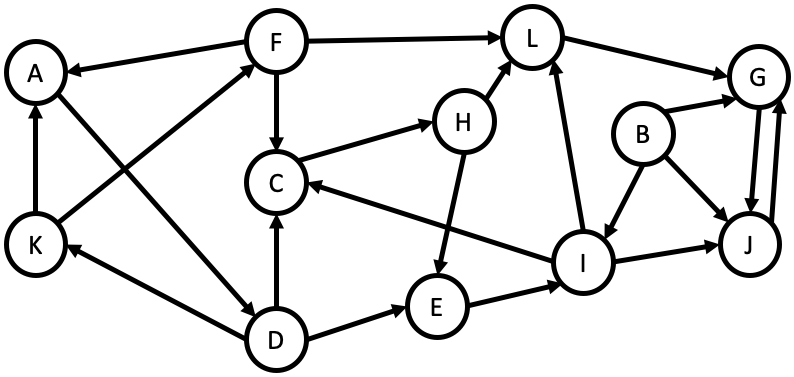
\includegraphics[scale=0.5]{img/scc.png}
    \end{center}

    \begin{parts}

        \part Is the graph a DAG?
        \begin{answer}
            No, $G \to J \to G$ is a cycle, hence it is not a DAG.
        \end{answer}

        \part How many SCCs does this graph have?
        \begin{answer}
            5
        \end{answer}

        \part How many source SCCs does this graph have?
        \begin{answer}
            2
        \end{answer}

        \part What is the distance of node $B$ from the node $A$?
        \begin{answer}
            Infinity, since there is no path from $A$ to $B$ (the indegree of $B$ is $0$ so there can be no path ending at $B$ with at least 1 edge).
        \end{answer}

        \part Suppose we run the DFS algorithm on the graph exploring nodes in alphabetical order. Given this, what is the pre-number of vertex $F$?
        \begin{answer}
            18
        \end{answer}

        \part Suppose we run the DFS algorithm on the graph exploring nodes in alphabetical order. Given this, what is the post-number of vertex $G$?
        \begin{answer}
            9
        \end{answer}
    \end{parts}

\question[7]
You are given a directed graph $G=(V,E)$ representing the map of a city where the nodes denote landmarks and directed edges denote one-way streets. The Mayor of the city is planning to construct Hospitals such that at least one of the Hospitals is reachable from any landmark in the city. To reduce cost, the Mayor wants to minimise the number of Hospitals. Design an algorithm that returns the minimum number of Hospitals that is required.

Assume that the graph is given in adjacency list representation. Design an algorithm for this problem. Give running time analysis and proof of correctness for your algorithm.

[Points distribution: Algorithm (3 points), proof of correctness (3 points), running time analysis (1 points)]

\begin{solution}

\textbf{Algorithm:}

    \begin{algorithmic}
        \Function{Solve}{$G$}
            \State let $G'$ := \Call{CreateMetaGraph}{$G$}
            \State let $count := 0$
            \For{$v \in V(G')$}
                \If{the adjacency list of $v$ is empty} \Comment{$v$ corresponds to a sink SCC in $G$}
                    \State $count := count + 1$
                \EndIf
            \EndFor
            \State \Return $count$
        \EndFunction
    \end{algorithmic}


\textbf{Proof:}

Note that in any strongly connected component $C$, if a hospital is reachable from vertex $v$ in $C$, then it is reachable from any other vertex $u$ in $C$.

Now I claim that it is necessary and sufficient to add one hospital per sink SCC.

Proof of necessity:

Since the outdegree of the sink SCC is $0$, there needs to be a hospital at a node in the SCC, because if there wasn't, then there is a path from this SCC to the SCC of the hospital which is reachable from this node, and thus this SCC has an outgoing edge in the metagraph, which is a contradiction since this is a sink SCC by definition.

Proof of sufficiency:

For any node in a sink SCC, there is a path from that node to the hospital in its SCC, by the definition of SCC.

For any other node $v$, I claim that there is always a path to a hospital in a sink SCC.

Consider the longest path in $G'$ emanating from the SCC of $v$. Suppose the last vertex on it is $u$. If $u$ is not a sink SCC, then there exists an SCC to which there is an edge, say $u'$. Then
    $u'$ is not on the path from $v$ to $u$, otherwise there would be a cycle. So $u'$ can be appended to the path from $v$ to $u$, to give an even longer path, which is a contradiction to the
    assumption that the path from $v$ to $u$ is the longest path emanating from $v$. Hence our assumption that $u$ is not a sink SCC is wrong, so $u$ is in fact a sink SCC. Hence we have shown by construction that there is a path from the SCC of any node to a sink SCC.

Now note that corresponding to this path in $G'$, there is a path from any node in the SCC of $v$ to any node in a sink SCC in $G$ (by concatenating paths within SCCs connecting the linking
    vertices/source/sink nodes with the linking edges between SCCs). In particular, since we put a hospital in any SCC, we find that there is a path from $v$ to a hospital, and thus we can conclude
    the proof of sufficiency.

This establishes my claim, and hence the minimum number of hospitals that need to be added are precisely the number of sink nodes in the metagraph of G. Our algorithm creates the metagraph and for
    each sink node in the metagraph (i.e., any node $v$ with no $u$ such that $(v, u)$ is an edge, i.e., a node with an empty adjacency list) it increments the count by $1$, and in the end, returns
    the count, which is also the number of sink SCCs in $G$, and thus our algorithm is correct.


\textbf{Time complexity analysis:}

Creating the metagraph can be done in $O(V + E)$ time. For the second loop, checking if a given vertex has no neighbours and incrementing count takes $O(1)$ time (if it is a linked list, we check if the
    head is a null node or not, and if the adjacency list of the node is implemented using a vector (dynamic array), we check whether the size is $0$ or not), hence the complexity of the second loop is
    $O(V')$ where $V'$ is the number of vertices in the metagraph of $G$. Returning the answer takes $O(1)$ time, so the overall complexity is $O(V + E + V')$ which is $O(V + E)$ as $V' \le V$
\end{solution}

\end{questions}
\end{document}

